\section{Results}
    \subsection{Magnetization vs. Temperature Results}
    The magnetization measurements for the a-axis of the sample is found in \autoref{fig:MvsT_a}. The magnetization for the b-axis is found in \autoref{fig:MvsT_b}. The magnetization of the c-axis is found in \autoref{fig:MvsT_c}. A comparison between the $\chi$ for the a and b axis for each temperature is found in \autoref{fig:a-b-difference}.
    From \autoref{fig:MvsT_a}, we can see that a splitting between ZFC and FC occurs, with the highest difference being 5.03e-6 emu/(cm³Oe)
    \begin{figure}
    \centering
    \begin{subfigure}{0.45\linewidth}
        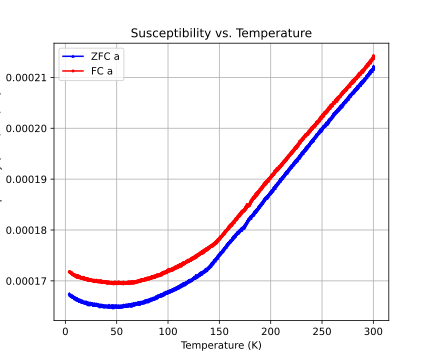
\includegraphics[width=\linewidth]{pdf_files/MvsT_a.pdf}
        \caption{M vs. T for the a-axis. FC-ZFC splitting is observed with FC displaying a higher susceptibility.}
        \label{fig:MvsT_a}
    \end{subfigure}
    \begin{subfigure}{0.45\linewidth}
        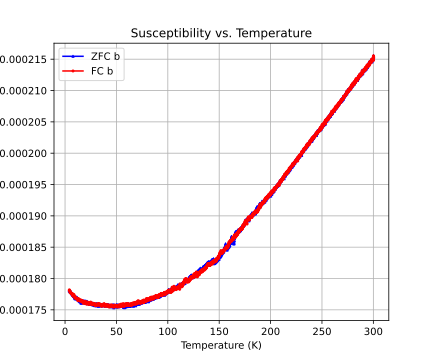
\includegraphics[width=\linewidth]{pdf_files/MvsT_b.pdf}
        \caption{M vs. T for the b-axis. No FC-ZFC splitting can be observed as any difference is within the error of measurement.}
        \label{fig:MvsT_b}
    \end{subfigure}
    \begin{subfigure}{0.45\linewidth}
        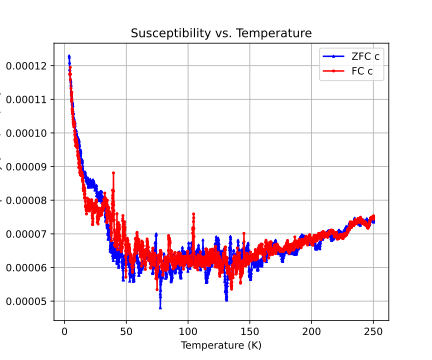
\includegraphics[width=\linewidth]{pdf_files/MvsT_c.pdf}
        \caption{M vs. T for the c-axis. Data very noisy due to thinness of sample in this orientation.}
        \label{fig:MvsT_c}
    \end{subfigure}
    
    \caption{M vs. T measurements for 3 different orientations, denoted a-axis, b-axis and c-axis respectively. The x-axes show the temperature measured in Kelvin, the y-axes the volume susceptibility measured in emu/cm³/Oe.}
    \label{fig:MvsT-tot}
\end{figure}
    


\begin{figure}
    \centering
    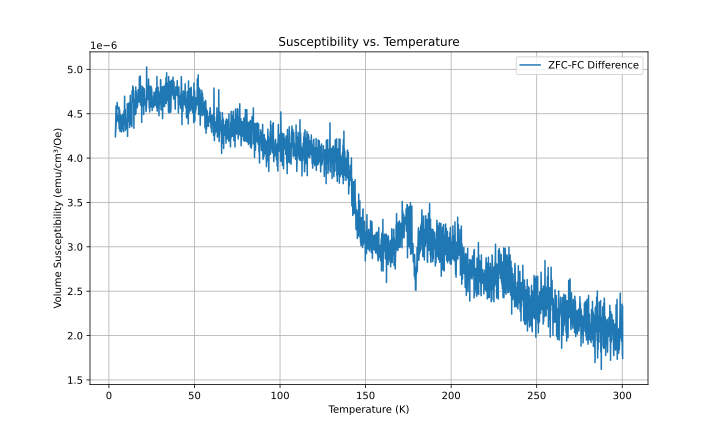
\includegraphics[width=\linewidth]{pdf_files/zfc_fc_a_difference.pdf}
    \caption{Difference in magnetic susceptibility between ZFC and FC for the a-axis. The average difference was found to be around 3.427e-06 emu/cm³/Oe. The x-axis shows the temperature measured in Kelvin, the y-axis the volume susceptibility measured in emu/cm³/Oe.}
    \label{fig:zfc-fc-a-difference}
\end{figure}
    %Show and describe your results here. \\ \\
    %Magnetization results + analysis \\ \\
    %Source of potential errors
    %

\begin{figure}
    \centering
    \includesvg[width=\linewidth]{svg_files/prelInverseMvsT.svg}
    \caption{Inverse of magnetic moment, which is proportional to magnetic susceptibility, plotted as function of temperature.}
    \label{fig:inverseMvsT}
\end{figure}



    \subsection{Magnetization vs. Magnetic Field Results}
    The M vs. H measurements were only done for the b- and c-axis, resulting in two very different graphs. The graph for M vs. H for the b-axis is found in \autoref{fig:MvsH-b}, while the M vs. H graph for the c-axis is found in figure \autoref{fig:MvsH-c}.
    

\begin{figure}
    \centering
    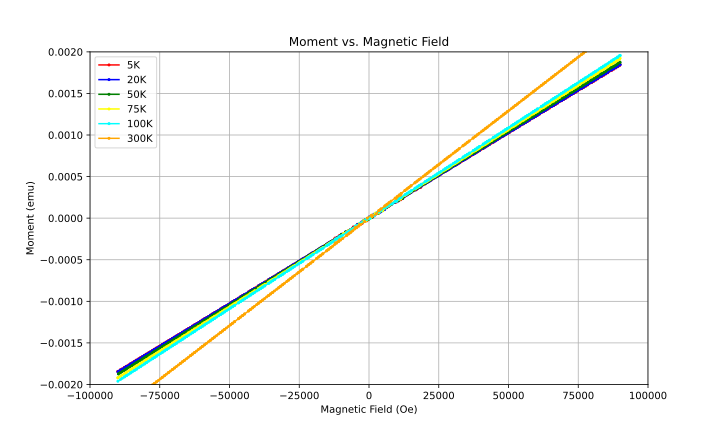
\includegraphics[width=\linewidth]{pdf_files/MvsH_all.pdf}
    \caption{M vs. H measurements for different temperatures along the b-axis. All R² values for linear fits of the data are 1.000 when using 4 significant figures, meaning the susceptibility is indeed linearly dependent on the applied field. The x-axis shows the magnetic field measured in Oe, while the y-axis shows the magnetic moment measured in emu.}
    \label{fig:MvsH-b}
\end{figure}

    

\begin{figure}
    \centering
    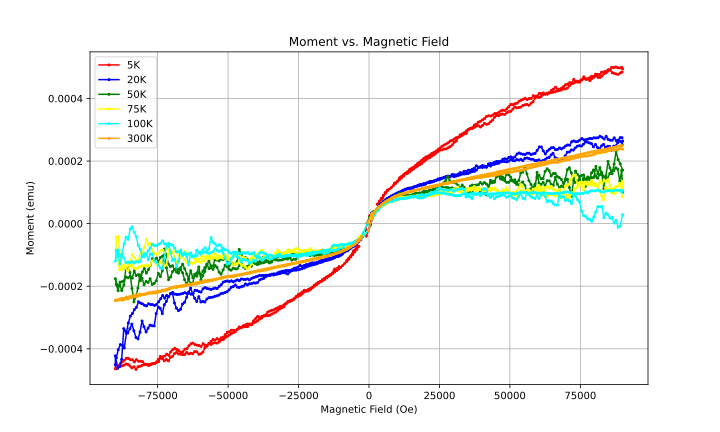
\includegraphics[width=\linewidth]{pdf_files/MvsH_c.pdf}
    \caption{M vs. H measurements for different temperatures along the c-axis. Unlike the b-axis, the magnetic moment was not linearly dependent on the magnetic field. The x-axis shows the magnetic field measured in Oe, while the y-axis shows the magnetic moment measured in emu.}
    \label{fig:MvsH-c}
\end{figure}


    \subsection{Analysis}
    By analysing the results, further conclusions about the magnetic properties of CrSb may be drawn.
    \subsubsection{Magnetic Anisotropy}
    By comparing the susceptibility as a function of temperature  between the a- and b-axis, it can be seen that CrSb is anisotropic due to the difference in magnetic susceptibility between different orientations of the material. Specifically, the b-axis shows a larger susceptibility and, unlike the a-axis, no splitting between the ZFC and FC measurements. The difference in susceptibility between the axes can be found in \autoref{fig:a-b-difference}. For data compiling the highest, lowest and average difference, see \autoref{tab:a-b-diff}. 


\begin{figure}
    \centering
    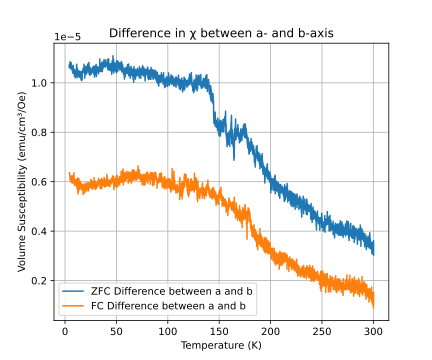
\includegraphics[width=\linewidth]{pdf_files/a_b_difference.pdf}
    \caption{The difference in susceptibility between the two main orientations, the a-axis and the b-axis. Both ZFC and FC differences were calculated. The x-axis shows the temperature measured in Kelvin, the y-axis the volume susceptibility measured in emu/cm³/Oe.}
    \label{fig:a-b-difference}
\end{figure}


    \begin{table}
    \centering
    \caption{Relevant data over the difference in susceptibility between the a-axis and b-axis.}
    \begin{tabular}{|c|c|c|}
         \hline
         Value& ZFC & FC \\
         \hline
         Highest Difference& 1.109e-05 emu/cm³/Oe &6.637e-06 emu/cm³/Oe\\
         Lowest Difference& 3.030e-06 emu/cm³/Oe&8.968e-07 emu/cm³/Oe\\
         Average Difference & 7.805e-06 emu/cm³/Oe & 4.357e-06 emu/cm³/Oe\\
         \hline
    \end{tabular}
    \label{tab:a-b-diff}
\end{table}
    \subsubsection{ZFC-FC Splitting}
    As mentioned, the measurements along the b-axis does not show any ZFC-FC splitting, but the a-axis does. The FC case shows a higher susceptibility. The difference in susceptibility between the ZFC and FC cases for the a-axis is found in \autoref{fig:zfc-fc-a-difference}.
    \subsubsection{Temperature Dependence}
    Both the a- and b-axis show an increasing susceptibility with increasing temperature. This does not follow the standard Curie-Weiss behaviour and thus requires us to use a modified version of it which includes a temperature independent term $\chi_0$ and a linear term $aT$, as described in Equation (\ref{eq:extended-curie-weiss}).
    \\ \\
    By using the python library \textit{Scipy}, a curve with the formula shown in Equation (\ref{eq:extended-curie-weiss}) can be fitted and values for $C$, $\theta_{CW}$, $\chi_0$ and $a$ can be found. However, creating a fit over the entire temperature range yields values for the parameters which are unphysical or a fit which does not fit the data that well. This can be resolved by restraining the fit to only be over a smaller part of the temperature range. The best suited range was found to be around the 50-300 K temperature range, which the fitted line in \autoref{fig:a-fitted-cw} is based around.
    \\ \\
    For our purposes, the Curie Constant $C$ is the most interesting. The fitted curve and constant $C$ for the a-axis is found in \autoref{fig:a-fitted-cw}. Using Equation (\ref{eq:u-eff}), the effective magnetic moment can be found with the help of the Curie Constant, see \autoref{tab:curie-const-mu-eff}. The magnetic moment for Cr\textsuperscript{3+} ions can be calculated from Equation (\ref{eq:free-ions-moment}) using $n=3$, which yields a magnetic moment for Cr\textsuperscript{3+} as $\mu_{eff}\approx3.87\mu_B$. 
    \\ \\
    The c-axis temperature dependence was different from the a-axis and b-axis. In particular, there appears to be a shoulder near the 5-25 K range, displaying a curve which starts with a rapid decrease in magnetization as the temperature increases, before leveling out and seeing an increase in magnetization with the increasing temperature. The c-axis does nor display any signs of ZFC-FC splitting outside the expected error due to the noise of the data.
    \begin{figure}
    \centering
    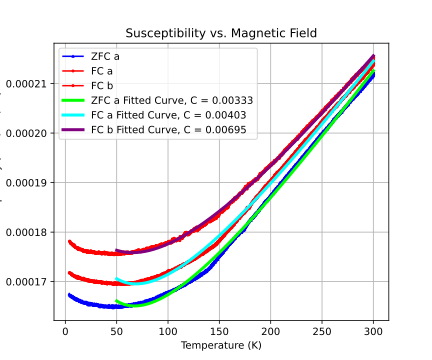
\includegraphics[width=\linewidth]{pdf_files/a_fitted_cw.pdf}
    \caption{ZFC a-axis, FC a-axis and FC b-axis data plotted together with fitted curves and extracted Curie Constant. The x-axis shows the temperature measured in Kelvin, the y-axis the volume susceptibility measured in emu/cm³/Oe.}
    \label{fig:a-fitted-cw}
\end{figure}
    \begin{table}
    \centering
    \caption{Extracted Curie Constants and effective magnetic moments measured in Bohr Magnetons. One standard deviation from the fitted data is specified.}
    \begin{tabular}{|c|c|c|}
        \hline
        Data&Curie Constant & Effective Moment $\mu_{eff}$ \\
        \hline
        ZFC a-axis & $0.003329\pm0.0001481$ & $0.163\mu_B$ \\
        %\hline
        FC a-axis&$0.004028\pm0.0001862$& $0.179\mu_B$ \\
        %\hline
        FC b-axis&$0.00695\pm0.0002583$& $0.236\mu_B$ \\
        \hline
    \end{tabular}
    \label{tab:curie-const-mu-eff}
\end{table}
    \subsubsection{Fitted Magnetization vs. Magnetic Field and Hysteresis}
    The M vs. H graphs plotted in \autoref{fig:MvsH-b} and \autoref{fig:MvsH-c} show that the b-axis and c-axis do not feature any magnetic hysteresis. The plots for all temperatures in the b-axis are completely linear and a fitted linear regression yields a R² value of 1.000 after rounding to 4 significant figures. The lack of hysteresis signifies either antiferromagnetic or paramagnetic behaviour. The graph for the c-axis is far more noisy. This is due to how thin the sample was in the c-axis, leading to a smaller registered magnetic moment which means that the noise has a higher impact on the measurements. The lines are noted to not be linear, however, no signs of a hysteresis loop can be seen. How thin the sample is also affects the contribution of the surface of the sample which, due to not being positioned within the crystal and some atoms missing neighbours, leads to different behaviour. 